%Intro, chapter 1 of ott/longnecker
\begin{center}\large\textbf{Readings: Chapter 1 (for 1.3 just read the 2 that interest you the most)}\\
\normalsize \end{center}
\large ~\hrulefill~\\~\\
\normalsize

\underbar{~~~~~~~~~~~~~~~~~~~~~~~~~} - the science of designing studies or experiments, collecting data and modeling/analyzing data for the purpose of decisions making and scientific discovery when the available information is both limited and variable.\\~\\

Why learn statistics?
\begin{itemize}
\item	We live in a society that collects volumes upon volumes of data.  
\item Are people looking at the data? 
\item	Are they interpreting the data properly?  
\item How do we turn raw data into information?
\begin{itemize}
\item	to make new policy
\item	to make better product
\item to increase yield
\end{itemize}
\end{itemize}

Statistics is often called the `science of learning from data.'\\~\\

\newpage

\textbf{ex: Gas mileage}\\
Suppose we fill 20 of the same model of car with a full tank of gas.  Each car will have a different miles per gallon.\\
Why?  \\~\\~\\~\\~\\~\\~\\~\\
\textbf{Factors} that affect gas mileage:\\~\\~\\~\\~\\~\\~\\~\\~\\~\\~\\
To summarize the information from the 20 cars we might look at the \textbf{average} gas mileage of the 20 cars.\\~\\
Questions to answer:
\begin{itemize}
\item How do we obtain an overall average miles per gallon for this model of car?  (Not just for these 20.)
\item	overall average when driving in city?
\item overall average when driving on a highway?
\item overall average with low tire pressure?
\item overall average when in a city with low tire pressure?
\end{itemize}
Statistics provides a framework for solving this type of problem!\\~\\~\\


\textbf{Method of statistics often follows a 4 step process}
\begin{itemize}
\item	Step 1: Identify the research objective
\item	Step 2: Collect the information needed to answer the questions
\item Step 3: Organize and summarize the information.
\item Step 4: Draw conclusions from the information.
\end{itemize}
(Repeat as necessary to answer research objective.)

\newpage

\textbf{Big ideas in stats:}\\
\begin{itemize}
\item \underbar{~~~~~~~~~~~~~~~~~~~~~~~~~~~~~~} - all the values, items, or individuals of interest\\~\\

\item \underbar{~~~~~~~~~~~~~~~~~~~~~~~~~~~~~~}  - a (usually) unknown summary value about the population\\~\\

\item \underbar{~~~~~~~~~~~~~~~~~~~~~~~~~~~~~~} - a subset of the population we observe data on\\~\\

\item \underbar{~~~~~~~~~~~~~~~~~~~~~~~~~~~~~~} - a summary value calculated from the sample observations
\end{itemize}
~\\~\\~\\~\\
\begin{center}
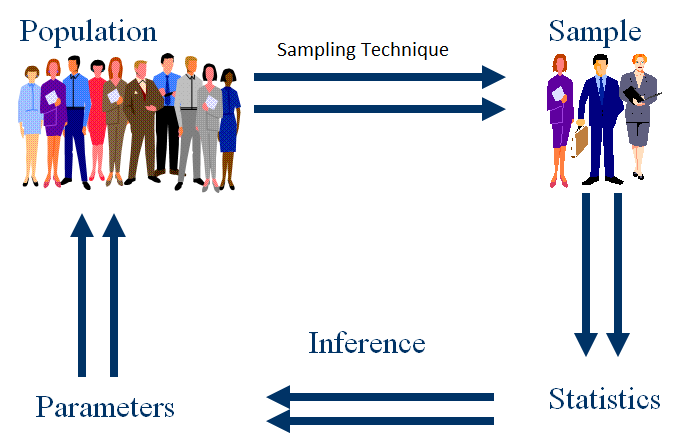
\includegraphics[scale=0.55]{paradigm}
\end{center}
~\\~\\~\\~\\
\textbf{Gas Example:}\\
What is the population, sample, parameter of interest, and statistic (most likely to be used)? 

\newpage

Common Notation in statistics:
\begin{center}
\begin{tabular}{c|ccc}
Name & Parameter & Statistic & Quantity Measured\\
\hline
&&&\\
Mean & $\mu$ & $\bar{Y}$ or $\bar{y}$ or $\bar{X}$ or $\bar{x}$ & Center or Location\\
&&&\\
Proportion & $p$ or $\pi$ & $\hat{P}$ or $\hat{p}$ or $\hat{\pi}$ & Location or Frequency\\
&&&\\
Standard Deviation (SD) & $\sigma$ & $S$ or $s$ & Variability or spread\\
&&&\\
Variance (Var) & $\sigma^2$ & $S^2$ or $s^2$ & Variability or spread\\
\end{tabular}
\end{center}
~\\
Note: $\bar{Y}=\frac{1}{n}\sum_{i=1}^{n}Y_i$ and $S^2=\frac{1}{n-1}\sum_{i=1}^{n}(Y_i-\bar{Y})^2$ where $n$ is the sample size (or number of observed values in the sample).\\~\\
Many, many, many, more to come! \\~\\~\\

Question of interest will lead you to which parameter you have interest in.  This will also most likely lead you to which type of data you will collect.\\~\\


\textbf{Scales (Types) of Data:}\\
\begin{itemize}
\item \underbar{~~~~~~~~~~~~~~~~~~~~~~~~~~~~~~~~~~~~~~~~~~~~~~~~~} - A variable that is described by attributes or labels\\
\indent Subscales: \\
Nominal - categories have no ordering (Male, Female) (zip codes)\\
Ordinal - can order categories (Lickert scale data) (college football rankings)\\~\\
\item \underbar{~~~~~~~~~~~~~~~~~~~~~~~~~~~~~~~} - A variable that is described by numerical measurements where arithmetic can be performed\\
\indent Subscales: \\
Discrete - finite or countable finite number of values (\# of flowers on a plant, 0, 1, 2, ...)\\
Continuous - any value in an interval is possible (Temperature, $(-459.67\deg F, \infty)$\\
(Some lump these together and call them interval.)
\end{itemize}
~\\
How we summarize and analyze the data will depend on which type of data we have.

\newpage

\textbf{ex: SAT (get to know each other a little!)}\\
\begin{itemize}
\item 50 total students (16 males and 34 females) where matched on socio-economic background (all had similar income). 
\item A study was done to examine the effect of preparation atmosphere on SAT scores.  
\item Two types of atmospheres were investigated (strict vs easy going).
\item Students were divided into two groups of 25 (12 males and 13 females in strict class and 4 males 21 females in the easy going class).
\item After a 9 week tutoring session the SAT was taken (although 1 in the strict group did not take the exam and 5 in the easy going group did not take the exam).
\end{itemize}
With a partner or two (introduce yourselves):
\begin{enumerate}
\item Determine the research question.
\item Define the population and sample.
\item Define possible parameter(s) of interest.
\item Define possible statistics that might be calculated.
\item Why might the students have been matched on socio-economic background?
\item What issues might you see with the design of this study?
\item What other variables might you collect?
\end{enumerate}